\documentclass{article}

\title{Estimating Comparative Advantage in Improved Seed Adoption: Hybrid Maize in Ethiopia}

\usepackage{natbib}
\bibliographystyle{rusnat}
\usepackage{multicol}
\usepackage{multirow}
\usepackage{booktabs}
\usepackage{caption}
\usepackage{amsmath}
\usepackage{longtable}

\usepackage{graphics}

\usepackage[margin=1in]{geometry}
\usepackage{setspace}
\doublespacing


\begin{document}

\maketitle

\begin{itemize}
    \item Tim Weiss- hybrid subsidies
    \item is there such a thing as traditional seeds?
    \item Let's evaluate the effect of adoption in the context of Ethiopia
    \item find ambiguous results, Why?
    \item have access to DNA fingerprinting data
    \item what do they say about adoption?
    \item turns out that "adoption" isn't really a reliable concept/variable
    \item most farmers are "adopting" under pretty conservative purity definitions
    \item Let's see what happens with different varieties of seed, does adoption of that seed lead to positive yield effects?
    \item can't use these methods but newer data has access to newer varieties where we're relatively more confident
\end{itemize}

\section{Introduction}

Food security is a major challenge in many East African countries-- Ethiopia is no exception, having historically struggled to provide an adequate and reliable food supply \citep{Ramakrishna2002-hv, Jaleta2018-oj}. Since the drought of 1984, Ethiopia has become increasingly reliant on maize, as of today, it constitutes the most widespread crop in the country.\footnote{FAO stats data shows the total area cultivated with Maize in 2019 is 25\% larger than the one cultivated with the next most widespread crop (sorghum), and 27\% and 139\% larger than the next two following crops, wheat and Barley, respectively.} As Figure \ref{fig:maize_yields} shows, there is an upward trend in the total area cultivated by maize, with average yields that have almost double during the period.

%%%%% The puzzle 
Despite numerous technological breakthroughs in maize germplasm with increased yields and drought tolerance, adoption of improved seed has remained a challenge, with only 13\% of maize farmers consistently using improved seeds varieties, and the lion share of farmers (62\%) not using improved seeds at all during the period where data is available. Moreover, there is a large percentage of farmers who adopt new varieties inconsistency limiting their opportunities to learn about their benefits, see Table \ref{tbl:Trajectories}. 


The facts sub-Saharan farmers continue to use traditional farming techniques when more modern, higher-return agricultural technologies are available remains an empirical puzzle where several answers have been proposed. These include imperfections in credit markets \citep{Croppenstedt2003-pq}, property rights \citep{Place2000-el}, social learning \citep{Conley2010-ue,Foster1995-bz,Munshi2004-og}, lack of commitment devices \cite{Duflo2009-iv}, and high transportation costs that increase the cost of agricultural inputs \citep{Byerlee2013-qk}. This issue is becoming more important as even current varieties of improved seed are over 20 years old and their effectiveness in terms of yield improvement and disease resistance is waning \citep{Abate2015-rj}. 

In this paper, we revisit the mechanism proposed by  \citep{Suri2011-oi} that justifies this lack of technology adoption on the existence of farmers heterogeneity. In particular, the fact that farmers with high net returns to the technology use new technologies while those with low returns do not. Adoption of a technology involves several dimensions such as market integration, access to supplementary inputs like fertilizer, as well agro-ecological considerations such as climate, altitude and soil quality. Ignoring the heterogeneity of these factors can hide the true impact of adoption, as different sub-populations may be impacted by the same technology in different, and even opposite ways. One way to tackle this problem, proposed by \citep{Suri2011-oi}, centers around quantifying the comparative advantage of a household to adopting improved seed varieties. Even when average returns are high, farmers may face heterogeneous returns based on their own, unobservable, comparative advantage in adopting new technologies. Using a correlated random coefficient model, Suri’s seminal paper finds that farmers’ lack of adoption is driven by insufficient net benefits to the technology stemming from poor infrastructure. Similar work in Ethiopia on improved chickpea varieties suggests that the economic returns to adoption plays a major role in the decision to adopt \citep{Michler2018-wk}.

In our paper, we build on that literature by investigating hybrid maize seed adoption in Ethiopia, focusing on how heterogeneous returns are also driven by climate and how this can affect dis-adoption decisions. We extend the role of heterogeneity in a household’s decision to adopt new technologies in four fronts. 

% We describe what we do here and what we find. We can expand as we have results
1) First, we test if the adoption of improved seed varieties takes place where the net benefits of adoption is highest? 

2) Second, we test how the adoption decision correlates with other adaptation strategies such as water storage, and irrigation augment a household’s comparative advantage in adoption.

3) Third. what are the drivers of dis-adoption of improved maize seed? and (4) is it possible to extend the methodology in \citep{Tjernstrom_Emilia_Dalia_Ghanem_Oscar_Barriga_Cabanillas_Travis_J_Lybbert_Jeffrey_D_Michler_and_Aleksandr_Michuda2020-bc} by including time-varying characteristics to the Group Random Coefficients (GRC) model?


% Persistent lack of adoption is a reflection of the distribution of (observable and unobservable) costs and benefits of the technology. The approach here models households’ adoption decisions in an environment with household-specific heterogeneity in the costs and benefits, and hence profits, to the technology. I estimate how the returns to the technology vary across farmers and then compare these returns to the adoption decisions of farmers. I find that farmers with low (or zero) returns to the technology are precisely the farmers who do not adopt it.  In particular, I use a generalized




\begin{figure}[H]
    \centering
    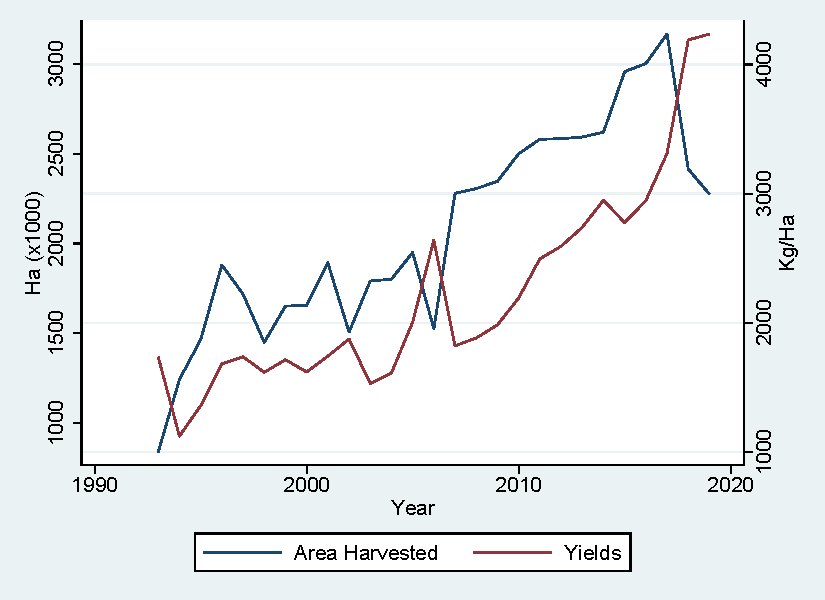
\includegraphics{results/figures/Maize_yields.pdf}
    \caption{Maize: Total area harvested and Average yields}
    \figcaption{Source: Authors' calculations using FAO stats data
    Note: Yield means the harvested production per ha for the area under cultivation}
    \label{fig:maize_yields}
\end{figure}


\section{Context}

Evidence has shown that the adoption of improved seed leads to increases in agricultural yields \citep{Carter2014-fm}, food security \citep{Shiferaw2014-op} and poverty reduction \citep{Minten2008-tj}. Despite such positive impacts, the low adoption levels of improved seeds varieties in Sub-Saharan Africa remains a puzzle. 


Multiple explanations have been proposed for observed adoption rates, including the type of technology promotion mechanisms used by governments, NGO’s, and businesses, the characteristics of the improved seeds and their adaptation to specific agro-climatic environments \citep{Bird2020-nt}, as well as growing conditions, such as the type of soil, input use, and other farmer characteristics \citep{Munshi2004-og}. The consensus in this literature is that the success of improved varieties depends on a range of factors that need to be better understood. Success of improved seeds should be accompanied by complementary conditions and inputs that would allow the full potential of these varieties to be realized. Specifically, extension services and on-farm field trials, seed variety characteristics and rainfall have been found to be crucial to the adoption of improved maize in Tanzania \citep{Kaliba2000-jh}. In the specific case of Ethiopia, labor, fertilizer use, farmers’ experience with extension packages, rainfall suitability and prices have been shown to increase the opportunity cost of not adopting improved wheat varieties \citep{Wale2006-bv}. Market access and the accessibility of extension services are also critical in the adoption of improved chickpea varieties in Ethiopia \citep{Verkaart2019-ol}. Other important determinants of heterogeneous effects include risk aversion \citep{Holden2016-vy}, farm size \citep{Ghimire2015-bd}, and credit constraints \citep{Simtowe2008-jn,Balana2020-hx}.



A different branch of the literature provides an alternative explanation for such low adoption rates, focusing on heterogeneous potential returns to adoption \citep{Suri2011-oi}. This literature suggests that even if returns to adoption are high, farmers may fail to adopt if they face low comparative advantage to adoption. Other methods used in the literature fail to account for this heterogeneity, admitting only the presence of time-constant and/or time-varying unobserved heterogeneities (depending on the data structure) for identification purposes \citep{Kassie2018-xn,Falco2011-rt}. These methods ignore the possibility of a farmer’s comparative advantage of using an improved technology over a traditional one as playing a central role in their adoption decision. 


We rely on Suri’s method and its extension in \citep{Tjernstrom_Emilia_Dalia_Ghanem_Oscar_Barriga_Cabanillas_Travis_J_Lybbert_Jeffrey_D_Michler_and_Aleksandr_Michuda2020-bc} to account for such heterogeneous comparative advantages and evaluate how these are explained by climatic conditions. In Ethiopia, rainfall deviations from historical averages are found to be the main driver of heterogeneous effects for adopting agronomic packages \citep{Marenya2020-kb}. Similar experiences from Malawi show exposure to past droughts is found to increase the adoption of drought-tolerant maize among farmers that also receive subsidies \citep{Katengeza2019-af} and the dis-adoption of traditional local maize \citep{Holden2016-vy}.

We will contribute to this literature by considering historical climate averages on the suitability of improved varieties to understand whether adoption is indeed realized where its potential is highest. Moreover, we will contribute to the understanding of how water conservation innovations and irrigation mitigate the effects of droughts on the potential of improved seeds.

\section{Data}

The current study uses the Ethiopia Socioeconomic Survey (ESS), a part of the Agricultural Sample Survey (AgSS), a survey designed to obtain production estimates for the major crops. The survey is a join effort of the the Central Statistics Agency of Ethiopia, the World Bank and CGIAR (Consortium of International Agricultural Research Centers) \citep{kosmowski2020shining} that aims at collecting information from a representative sample of households in the  the most populous regions of the country. The ESS contains several questionnaires targeted at getting an understanding of the state of agriculture. This includes a survey that is conducted post-planting and then post-harvest. These surveys are more important to our analysis as it gives a close look to inputs used in agriculture, the types of seeds used (in various levels of detail) and yields collected post-harvest.

There were significant differences between the analysis carried out in ESS 1-3 and the most recent, ESS4. Most notably, the ESS4 is no longer a panel dataset made up of the households of ESS 1-3, but it includes important information on the DNA fingerprinting of seed type and misclassification rates. This is important information as the first three waves of ESS only included self-reported hybrid maize status. Since our estimation strategy requires a balanced panel dataset of maize growers, our main analysis will include the first three waves of the ESS. We use the fourth wave later for robustness and validation.

Figure \ref{map:regions} shows the spatial distribution of the locations of the our households of study. As previously mentioned these are households that grow either improved or conventional maize and that are observed for all three rounds of the survey. Most households come from the northwest region of Amhara, Tigray and Oromiya which is consistent with where maize is mostly grown in Ethiopia \citep{Abate2015-rj}.

\begin{figure}
    \centering
    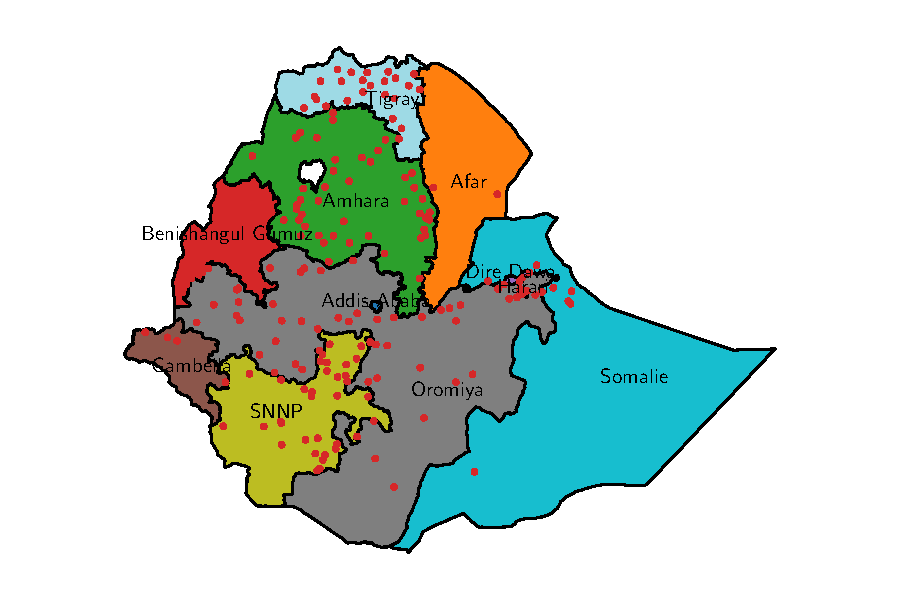
\includegraphics{results/figures/map_hhids.pdf}
    \caption{Spatial Distribution of Households Surveyed}
    \figcaption{Note: Green markers denote the locations of households}
    \label{map:regions}
\end{figure}

Table \ref{tbl:summary} shows a set of summary statistics for our sample. The mean parcel size for a household is about 0.15 Ha, with a maximum size of a little less than 1.5 Ha. Harvest labor is disproportionately skewed to family participation with around 20 days of harvest labor being conducted by family members and only about 2 days for hired labor. This is indicative of either malfunctioning labor markets, income constraints or high supervision costs. The distances to some key areas are also highlighted in Table \ref{tbl:summary}. On average households are around 13 kilometers away from an asphalt road and almost 60 kilometers away from the nearest market. This makes both the purchase of improved seed and the marketing of yields subject to transportation costs and a difficult enterprise. Fertilizer costs are on average 8,350 Birr (~178 USD) and with a large amount of the sample not using fertilizer at all. This is particularly important in the context of improved maize seed use as it requires fertilizer to be most effective. Only 5\% of the sample irrigates their crops making households susceptible weather shocks.

\begin{table}
\centering
\caption{Summary Statistics for Households}
\label{tbl:summary}
\begin{tabular}{lllll}
\toprule
                             & Wave &       1.0 &       2.0 &       3.0 \\
\midrule
Parcel Size & N &  1,116.00 &  1,116.00 &  1,116.00 \\
                             & Mean &      0.31 &      0.32 &      0.30 \\
                             & Std. Dev. &      0.36 &      0.39 &      0.35 \\
Household Labor for Harvest (Days) & N &  1,116.00 &  1,116.00 &  1,116.00 \\
                             & Mean &     45.51 &     38.29 &     36.33 \\
                             & Std. Dev. &     71.11 &     54.58 &     46.56 \\
Hired Labor for Harvest (Days) & N &  1,116.00 &  1,116.00 &  1,116.00 \\
                             & Mean &      4.27 &      3.38 &      4.89 \\
                             & Std. Dev. &     25.93 &     17.08 &     54.11 \\
Age of Household Head & N &  1,106.00 &  1,086.00 &  1,102.00 \\
                             & Mean &     43.85 &     45.91 &     48.23 \\
                             & Std. Dev. &     14.31 &     14.17 &     14.33 \\
Sex of Household Head & N &  1,109.00 &  1,114.00 &  1,108.00 \\
                             & Mean &      1.15 &      1.15 &      1.16 \\
                             & Std. Dev. &      0.36 &      0.36 &      0.36 \\
Years of Education of Household Head & N &  1,106.00 &  1,085.00 &  1,102.00 \\
                             & Mean &      1.46 &      1.56 &      1.64 \\
                             & Std. Dev. &      2.71 &      2.77 &      2.92 \\
Total Rainfall (mm) & N &  1,113.00 &  1,088.00 &  1,106.00 \\
                             & Mean &    899.23 &    953.98 &    943.03 \\
                             & Std. Dev. &    240.43 &    237.46 &    267.07 \\
Does Household have Title to land? & N &  1,113.00 &  1,088.00 &  1,106.00 \\
                             & Mean &      0.43 &      0.52 &      0.61 \\
                             & Std. Dev. &      0.50 &      0.50 &      0.49 \\
Crop Cut Dry Yield (kg/ha) & N &  1,105.00 &  1,103.00 &  1,103.00 \\
                             & Mean &     86.51 &    251.69 &    438.42 \\
                             & Std. Dev. &    200.25 &    532.17 &    786.49 \\
Self-reported Yields (kg/ha) & N &  1,043.00 &  1,075.00 &  1,064.00 \\
                             & Mean &    187.18 &  1,314.04 &  1,224.65 \\
                             & Std. Dev. &    435.03 &  1,157.66 &  1,105.53 \\
\bottomrule
\multicolumn{6}{l}{Note: Parcel size, yield and distance variables winsorized at the 1\% level.}
\end{tabular}
\end{table}


The ESS has has both self-reported and crop cut yields available. This provides two sources of yield information, although self-reported yields seem to be overly large compared to either fresh or dried crop cut yields. Self-reported yields are both more susceptible to behavioral biases, but also to confusion caused by differences in assumed units. In general, though, the sample with available yield information cuts down the available sample immensely, which limits the power of the estimation. It isn't clear whether unavailable yields numbers is due to some sort of selection or whether crop cuts were only collected randomly from a few households.

\begin{figure}
    \centering
    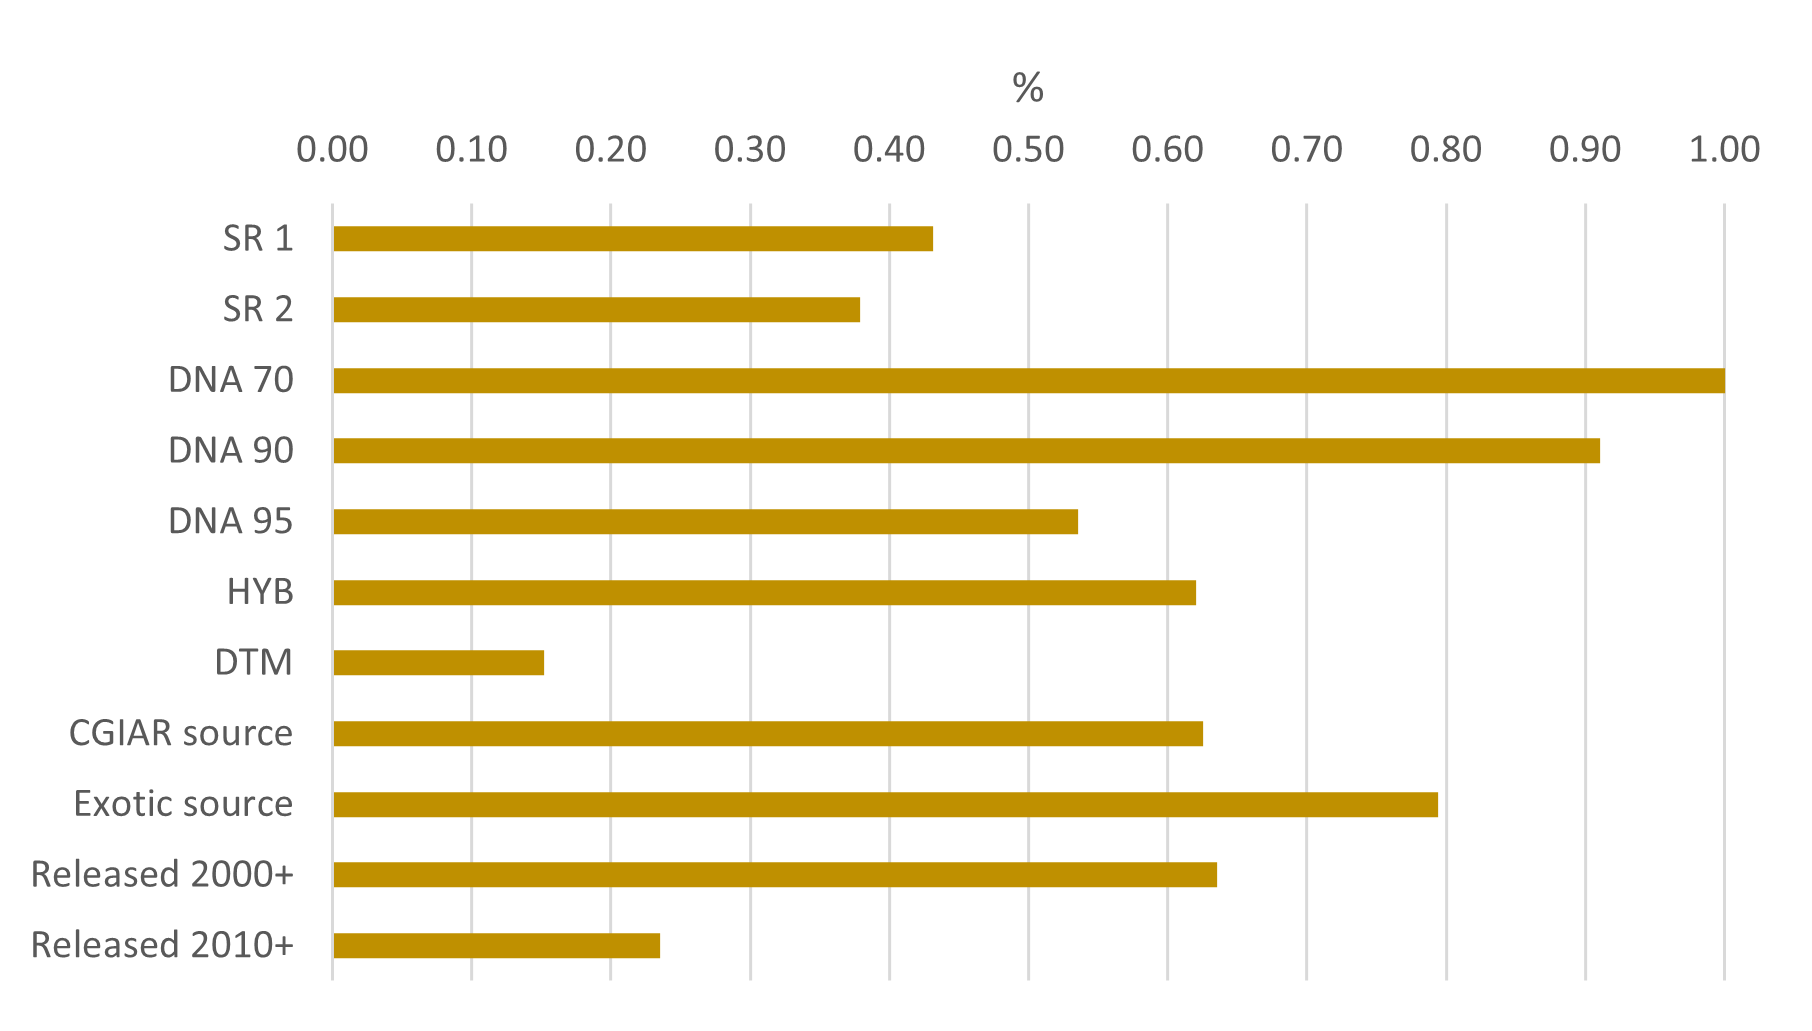
\includegraphics{results/figures/adoption_r4.png}
    \caption{Adoption rates of improved varieties in 2018 (by self-report, purity level, crop type, source and year of release)}
    \figcaption{Note: Shares represent the proportion of adopters among maize farmers. Acronyms include: SR1 - Self reported 1 [=1 if New, 2nd gen or recycled, =0 if Traditional]; SR2 - Self reported 1 [=1 if New, 2nd gen or recycled, =0 if Traditional]; DNA70 - Improved if purity $>=$70$\%$; DNA90 - Improved if purity $>=$90$\%$; DNA95 - Improved if purity $>=$95$\%$; HYB - Improved DNA, [=1 Hybrid, 0=Open pollinated]; DTM - Drought tolerant Maize [=1 DTM, 0=otherwise], CGIAR source [=1 if germplasm associated to a CGIAR-related thread], Exotic source [=1 if germplasm associated to an exotic source], Released 2000+ [=1 if DNA associated to a variety released on year 2000 or later], Released 2010+ [=1 if DNA associated to a variety released on year 2010 or later]. QPM is not included as there are too few households planting QPM seeds (n=6).}
    \label{fig:adoption_r4}
\end{figure}

\section{Estimation Strategy}

The advantage of our estimation strategy is that we do not rely on identification from an instrument or the structure of a model, but from the fact that the trajectory that a household takes in their adoption decisions through time is an informative source of identifying information. See \cite{Tjernstrom_Emilia_Dalia_Ghanem_Oscar_Barriga_Cabanillas_Travis_J_Lybbert_Jeffrey_D_Michler_and_Aleksandr_Michuda2020-bc} for more information on the assumptions involved for the Group Random Coefficients estimator. 

Table \ref{tbl:Trajectories} maps out the frequencies of the different trajectories present in the data, sorted by frequency. The largest portion of the data are those that do not adopt improved maize seed at all, followed with sharp decline, to those that use improved maize seed in every period. Interestingly, adoption trajectories seem to be more popular for later adoptions than earlier ones.



\begin{table}
\centering
\caption{Trajectories of Households}
\label{tbl:trajectories}
\begin{tabular}{lrr}
\toprule
Trajectory &  Frequency &    Share \\
\midrule
       000 &       2124 & 0.611927 \\
       111 &        456 & 0.131374 \\
       011 &        228 & 0.065687 \\
       001 &        219 & 0.063094 \\
       010 &        153 & 0.044080 \\
       100 &        108 & 0.031115 \\
       110 &         96 & 0.027658 \\
       101 &         87 & 0.025065 \\
\bottomrule
\multicolumn{3}{l}{Note: Table shows frequency and shares of each trajectory in sample. 1 denotes adoption and 0 otherwise. The first digit is for whether the household adopted in wave 1, the second digit for wave and the third digit for wave 3}
\end{tabular}
\end{table}


This method seeks to estimate the following equation:

\begin{align}
y_{it}&=\sum_{\underline{h}\in\mathcal{H}\backslash (1,1)}\mu_{\underline{h}}1\{h_{i}=\underline{h}\}+\sum_{\underline{h}\in\mathcal{H}_{S}}\Delta_{\underline{h}}h_{it}1\{h_{i}=\underline{h}\}+\kappa_{(1,1)}h_{it}1\{\underline{h}=(1,1)\}+\epsilon_{it}.\label{eq:GRC}
\end{align}

where y is yields or profits for household i at time t, h is an indicator for adoption,  is a household’s absolute advantage,  is a household’s comparative advantage and  describes the gains to adopting, relative to a household’s comparative advantage. This framework provides an advantage over other methods \citep{Wooldridge1997-xj,Heckman1998-pt}. Firstly, identification does not rely on the existence of a valid instrumental variable. Instead, identification comes from a linear projection of an individual's returns to adoption onto the observed history of their adoption, an approach similar to the correlated random effects (CRE) method in \citep{Chamberlain1984-uk}. Secondly, it disentangles a household’s absolute advantage when taking part in agriculture and its comparative advantage in adopting. This is crucial in understanding the adoption decision as it is not dependent on a household’s agricultural ability, but on the gains from taking it up. We and co-authors developed this further in \citep{Tjernstrom_Emilia_Dalia_Ghanem_Oscar_Barriga_Cabanillas_Travis_J_Lybbert_Jeffrey_D_Michler_and_Aleksandr_Michuda2020-bc} by proposing a more flexible and tractable approach using a group random coefficient strategy that draws on recent developments in the nonparametric panel identification literature. Our strategy has a clear economic interpretation and can elucidate potential identification concerns of the CRC model to the practitioner. It is also more easily extended to multiple time periods and new levels of heterogeneity than the CRC approach.

Estimating equation 1 will allow us  to analyze the distribution of the gains to adoption and to create a distribution of heterogeneous returns. We will investigate whether comparative advantage is driven by two key policy relevant factors: water conservation strategies and deviation from historical climate averages. The first will elucidate if adaptation strategies in water management are associated with higher levels of gains to adoption. The second will seek to understand whether households are adapting to climate change through their adoption decisions. This will require the extension of the method developed in \citep{Tjernstrom_Emilia_Dalia_Ghanem_Oscar_Barriga_Cabanillas_Travis_J_Lybbert_Jeffrey_D_Michler_and_Aleksandr_Michuda2020-bc}, by allowing for time-varying characteristics in the identification of comparative advantage.

Implications 

Our work has far-reaching policy implications. The adoption and impact of agricultural technologies is inherently heterogeneous. Our methodology incorporates that from the outset, allowing us to investigate whether synergies between seed adoption and water conservation strategies interact; a key component to understanding how investment into such projects translates to economic returns. Moreover, our research informs on not only the adoption but also dis-adoption decisions of technologies as well. In this sense, we provide valuable information to policymakers on how to better target seed marketing or infrastructure to help agricultural households improve their livelihoods

\section{Results}

{
\def\sym#1{\ifmmode^{#1}\else\(^{#1}\)\fi}
\begin{tabular}{l*{3}{c}}
\hline\hline
          &\multicolumn{1}{c}{(1)}&\multicolumn{1}{c}{(2)}&\multicolumn{1}{c}{(3)}\\
          &\multicolumn{1}{c}{Log Dry Cropcuts}&\multicolumn{1}{c}{Log Dry Cropcuts}&\multicolumn{1}{c}{Log Dry Cropcuts}\\
\hline
$\mu_{000}$&    6.350\sym{***}&    1.075\sym{***}&    5.849\sym{***}\\
          & (0.0372)         &  (0.132)         &  (0.202)         \\
$\mu_{001}$&    6.246\sym{***}&    0.720\sym{***}&    5.771\sym{***}\\
          &  (0.121)         &  (0.209)         &  (0.231)         \\
$\mu_{010}$&    6.405\sym{***}&    1.166\sym{***}&    6.049\sym{***}\\
          &  (0.151)         &  (0.301)         &  (0.259)         \\
$\mu_{011}$&    5.518\sym{***}&    0.218         &    5.324\sym{***}\\
          &  (0.207)         &  (0.496)         &  (0.310)         \\
$\mu_{100}$&    6.479\sym{***}&    1.002\sym{***}&    5.798\sym{***}\\
          &  (0.145)         &  (0.270)         &  (0.254)         \\
$\mu_{101}$&    6.466\sym{***}&    0.347         &    5.654\sym{***}\\
          &  (0.193)         &  (0.407)         &  (0.309)         \\
$\mu_{110}$&    6.908\sym{***}&    1.546\sym{***}&    6.271\sym{***}\\
          &  (0.277)         &  (0.401)         &  (0.335)         \\
$\Delta_{001}$&    0.634\sym{***}&    1.067\sym{***}&   -5.395\sym{***}\\
          &  (0.241)         &  (0.330)         &  (0.322)         \\
$\Delta_{010}$&   0.0398         &   -0.964\sym{**} &   -6.405\sym{***}\\
          &  (0.318)         &  (0.461)         &  (0.403)         \\
$\Delta_{011}$&    1.308\sym{***}&    1.137\sym{**} &   -5.100\sym{***}\\
          &  (0.249)         &  (0.519)         &  (0.342)         \\
$\Delta_{100}$&   -0.699\sym{***}&   -0.984\sym{**} &   -6.364\sym{***}\\
          &  (0.252)         &  (0.389)         &  (0.294)         \\
$\Delta_{101}$&    0.112         &    1.183\sym{***}&   -5.381\sym{***}\\
          &  (0.321)         &  (0.422)         &  (0.388)         \\
$\Delta_{110}$&   -0.302         &   0.0558         &   -6.376\sym{***}\\
          &  (0.304)         &  (0.395)         &  (0.354)         \\
\hline
Observations&      984         &      930         &      930         \\
Controls  &       No         &      Yes         &      Yes         \\
Interact w/ Hybrid&       No         &       No         &      Yes         \\
\hline\hline
\multicolumn{4}{l}{\footnotesize Standard errors in parentheses}\\
\multicolumn{4}{l}{\footnotesize \sym{*} \(p<0.10\), \sym{**} \(p<0.05\), \sym{***} \(p<0.01\)}\\
\end{tabular}
}


\begin{tabular}{llll}
\toprule
{} &           Base &      Controls & Controls w/ Int. \\
\midrule
Restriction 001-010 &      (-$\infty$, $\infty$) &     (-$\infty$, $\infty$) &        (-$\infty$, $\infty$) \\
Restriction 001-011 &   (-1.81, .01) &     (-$\infty$, $\infty$) &        (-$\infty$, $\infty$) \\
Restriction 001-100 &      (-$\infty$, $\infty$) &     (-$\infty$, $\infty$) &        (-$\infty$, $\infty$) \\
Restriction 001-101 &      (-$\infty$, $\infty$) &     (-$\infty$, $\infty$) &        (-$\infty$, $\infty$) \\
Restriction 001-110 &  (-7.11, -.49) &   (-$\infty$, -.02) &        (-$\infty$, $\infty$) \\
\hline\\Joint Test  &         $\emptyset$ &  (-$\infty$, -2.32) &     (-$\infty$, -1.92) \\
\bottomrule
\end{tabular}


{
\def\sym#1{\ifmmode^{#1}\else\(^{#1}\)\fi}
\begin{tabular}{l*{3}{c}}
\hline\hline
          &\multicolumn{1}{c}{(1)}&\multicolumn{1}{c}{(2)}&\multicolumn{1}{c}{(3)}\\
          &\multicolumn{1}{c}{Log Dry Cropcuts}&\multicolumn{1}{c}{Log Dry Cropcuts}&\multicolumn{1}{c}{Log Dry Cropcuts}\\
\hline
$\mu_{000}$&    6.587\sym{***}&    1.110\sym{***}&    6.444\sym{***}\\
          & (0.0310)         &  (0.144)         &  (0.134)         \\
$\mu_{001}$&    6.659\sym{***}&    1.261\sym{***}&    6.622\sym{***}\\
          &  (0.103)         &  (0.198)         &  (0.159)         \\
$\mu_{010}$&    6.942\sym{***}&    1.177\sym{***}&    6.835\sym{***}\\
          &  (0.118)         &  (0.229)         &  (0.186)         \\
$\mu_{011}$&    5.968\sym{***}&    0.518         &    5.930\sym{***}\\
          &  (0.363)         &  (0.459)         &  (0.393)         \\
$\mu_{100}$&    6.759\sym{***}&    1.551\sym{***}&    6.685\sym{***}\\
          &  (0.114)         &  (0.248)         &  (0.173)         \\
$\mu_{101}$&    7.011\sym{***}&    1.292\sym{***}&    6.838\sym{***}\\
          &  (0.166)         &  (0.327)         &  (0.213)         \\
$\mu_{110}$&    7.120\sym{***}&    1.520\sym{***}&    6.983\sym{***}\\
          &  (0.124)         &  (0.289)         &  (0.180)         \\
$\Delta_{001}$&    0.209         &   -0.180         &   -7.050\sym{***}\\
          &  (0.152)         &  (0.182)         &  (0.202)         \\
$\Delta_{010}$&   0.0531         &    0.191         &   -7.174\sym{***}\\
          &  (0.138)         &  (0.163)         &  (0.207)         \\
$\Delta_{011}$&    1.241\sym{***}&    1.024\sym{**} &   -6.002\sym{***}\\
          &  (0.380)         &  (0.468)         &  (0.412)         \\
$\Delta_{100}$&    0.718\sym{***}&    0.678         &   -6.484\sym{***}\\
          &  (0.136)         &  (0.572)         &  (0.205)         \\
$\Delta_{101}$&    0.157         &   -0.214         &   -6.984\sym{***}\\
          &  (0.262)         &  (0.342)         &  (0.299)         \\
$\Delta_{110}$&   -0.421\sym{***}&   -0.281         &   -7.497\sym{***}\\
          &  (0.158)         &  (0.189)         &  (0.233)         \\
\hline
Observations&     2320         &     2289         &     2289         \\
Controls  &       No         &      Yes         &      Yes         \\
Interact w/ Hybrid&       No         &       No         &      Yes         \\
\hline\hline
\multicolumn{4}{l}{\footnotesize Standard errors in parentheses}\\
\multicolumn{4}{l}{\footnotesize \sym{*} \(p<0.10\), \sym{**} \(p<0.05\), \sym{***} \(p<0.01\)}\\
\end{tabular}
}


\begin{tabular}{llll}
\toprule
{} &           Base &        Controls & Controls w/ Int. \\
\midrule
Restriction 001-010 &      (-$\infty$, $\infty$) &  (-3.37, -1.33) &      (-$\infty$, -.49) \\
Restriction 001-011 &      (-$\infty$, $\infty$) &       (-$\infty$, $\infty$) &        (-$\infty$, $\infty$) \\
Restriction 001-100 &      (-$\infty$, $\infty$) &       (-$\infty$, $\infty$) &        (-$\infty$, $\infty$) \\
Restriction 001-101 &    (-1.34, $\infty$) &       (-$\infty$, $\infty$) &        (-$\infty$, $\infty$) \\
Restriction 001-110 &  (-3.37, -.56) &    (-$\infty$, -1.27) &   (-5.84, -1.07) \\
\hline\\Joint Test  &         $\emptyset$ &  (-4.91, -1.34) &     (-$\infty$, -1.95) \\
\bottomrule
\end{tabular}


\begin{table}[H]
\centering
\hspace*{-1.2cm}
\begin{threeparttable}
\caption{Effects on yields (log) from adopting improved maize varieties (self-reported)}
\label{tab:switch1}
\begin{tabular}{l cccccc}
\hline
\hline
            &Adopters yields&Non-adopters yields&         ATE&          SE&     p-value\\
\hline
\textit{SR1, SR yields}&            &            &            &            &            \\
ATT         &        7.30&        9.07&       -1.76&       0.011&      0.0000\\
%
%
%
ATU         &        9.06&        6.87&        2.19&       0.024&      0.0000\\
%
%
%
\textit{SR1, cropcut yields}&            &            &            &            &            \\
ATT         &        7.57&        7.86&       -0.30&       0.017&      0.0000\\
%
%
%
ATU         &        8.89&        7.11&        1.78&       0.039&      0.0000\\
%
%
%
\textit{SR1, SR yields, full set of controls}&            &            &            &            &            \\
ATT         &        7.28&        7.82&       -0.54&       0.019&      0.0000\\
%
%
%
ATU         &        9.65&        6.85&        2.80&       0.100&      0.0000\\
%
%
%
\textit{SR1, cropcut yields, full set of controls}&            &            &            &            &            \\
ATT         &        7.56&        7.61&      -0.049&       0.019&      0.0087\\
%
%
%
ATU         &        9.24&        7.11&        2.13&       0.085&      0.0000\\
%
%
%
\textit{SR2, SR yields}&            &            &            &            &            \\
ATT         &        7.30&        7.85&       -0.55&       0.020&      0.0000\\
%
%
%
ATU         &        9.63&        6.88&        2.75&       0.101&      0.0000\\
%
%
%
\textit{SR2, cropcut yields}&            &            &            &            &            \\
ATT         &        7.61&        7.62&      -0.013&       0.019&        0.47\\
%
%
%
ATU         &        9.35&        7.14&        2.21&       0.091&    1.6e-130\\
\hline
\hline
\end{tabular}
\begin{tablenotes}
\footnotesize
\item{Note: Full set of controls include: parcel size (in HA), household labor, hired labor, fertilizer costs, other input costs irrigation (dummy), mechanization (dummy), organic fertilizer (dummy). Instruments for the adoption equation include: years of education of hh head, age of hh head, female head, land title, asset index, seed costs. Results for SR2 include full set of controls. SR1=1 if New, 2nd gen or recycled,=0 if Traditional; SR2=1 if New, =0 2nd gen, recycled or traditional}
\end{tablenotes}
\end{threeparttable}
\end{table}

\begin{table}[H]
\centering
\hspace*{-1.2cm}
\begin{threeparttable}
\caption{Effects on yields (log) from adopting improved maize varieties (DNA fingerprinting)}
\label{tab:switch2}
\begin{tabular}{l cccccc}
\hline
\hline
            &Adopters yields&Non-adopters yields&         ATE&          SE&     p-value\\
\hline
\textit{DNA 70, SR yields}&            &            &            &            &            \\
ATT         &        7.17&        7.31&       -0.14&       0.026&      0.0000\\
%
%
%
ATU         &        8.76&        6.76&        2.00&       0.036&      0.0000\\
%
%
%
\textit{DNA 70, cropcut yields}&            &            &            &            &            \\
ATT         &        7.28&        8.48&       -1.21&       0.041&      0.0000\\
%
%
%
ATU         &        8.55&        7.27&        1.28&       0.042&      0.0000\\
%
%
%
\textit{DNA 90, SR yields}&            &            &            &            &            \\
ATT         &        7.18&        9.07&       -1.90&       0.023&      0.0000\\
%
%
%
ATU         &        7.01&        6.80&        0.21&       0.022&      0.0000\\
%
%
%
\textit{DNA 90, cropcut yields}&            &            &            &            &            \\
ATT         &        7.30&        8.72&       -1.43&       0.028&      0.0000\\
%
%
%
ATU         &        9.32&        7.24&        2.09&       0.034&      0.0000\\
%
%
%
\textit{DNA 95, SR yields}&            &            &            &            &            \\
ATT         &        7.30&        7.08&        0.22&       0.036&      0.0000\\
%
%
%
ATU         &        6.87&        6.86&       0.018&       0.029&      0.5496\\
%
%
%
\textit{DNA 95, cropcut yields}&            &            &            &            &            \\
ATT         &        7.52&        7.39&        0.13&       0.018&      0.0000\\
%
%
%
ATU         &        7.38&        7.12&        0.26&       0.024&      0.0000\\
%
%
%
\textit{HYB, SR yields}&            &            &            &            &            \\
ATT         &        7.28&        7.25&       0.030&       0.028&      0.2892\\
%
%
%
ATU         &        7.06&        6.85&        0.21&       0.028&      0.0000\\
%
%
%
\textit{HYB, cropcut yields}&            &            &            &            &            \\
ATT         &        7.51&        7.55&      -0.038&       0.017&      0.0289\\
%
%
%
ATU         &        7.58&        7.03&        0.55&       0.021&      0.0000\\
%
%
%
\textit{DTMZ, SR yields}&            &            &            &            &            \\
ATT         &        7.42&        6.53&        0.89&       0.074&      0.0000\\
%
%
%
ATU         &        7.11&        7.02&       0.089&       0.022&      0.0001\\
%
%
%
\textit{DTMZ, cropcut yields}&            &            &            &            &            \\
ATT         &        7.56&        6.76&        0.81&       0.058&     3.5e-44\\
%
%
%
ATU         &        8.04&        7.27&        0.77&       0.028&    9.4e-167\\
\hline
\hline
\end{tabular}
\begin{tablenotes}
\footnotesize
\item{Note: Full set of controls include: parcel size (in HA), household labor, hired labor, fertilizer costs, other input costs irrigation (dummy), mechanization (dummy), organic fertilizer (dummy). Instruments for the adoption equation include: years of education of hh head, age of hh head, female head, land title, asset index, seed costs. All results include full set of controls. DNA 70, 90 and 95 refer to improved varieties defined by DNA finerprinting with purity levels of 70, 90 and 95\%, respectively. HYB equals 1 for a hybrid variety, 0 for an open-pollinated variety. DTMZ equals 1 for a Drought-tolerant maize variety}
\end{tablenotes}
\end{threeparttable}
\end{table}

\begin{table}[H]
\centering
\resizebox{0.8\textwidth}{!}{
\hspace*{-1.2cm}
\begin{threeparttable}
\caption{Effects on yields (log) from adopting improved maize varieties (DNA fingerprinting)}
\label{tab:switch3}
\begin{tabular}{l cccccc}
\hline
\hline
            &Adopters yields&Non-adopters yields&         ATE&          SE&     p-value\\
\hline
\textit{CGIAR source, SR yields}&            &            &            &            &            \\
ATT         &        7.13&        6.71&        0.43&       0.033&      0.0000\\
%
%
%
ATU         &        9.19&        6.89&        2.31&       0.018&      0.0000\\
%
%
%
\textit{CGIAR source, cropcut yields}&            &            &            &            &            \\
ATT         &        7.23&        8.98&       -1.75&       0.040&      0.0000\\
%
%
%
ATU         &        7.51&        7.40&        0.11&       0.015&      0.0000\\
%
%
%
\textit{Exotic source, SR yields}&            &            &            &            &            \\
ATT         &        7.13&        6.65&        0.48&       0.022&      0.0000\\
%
%
%
ATU         &        6.83&        6.89&      -0.060&       0.021&      0.0047\\
%
%
%
\textit{Exotic source, cropcut yields}&            &            &            &            &            \\
ATT         &        7.28&        7.18&       0.098&       0.032&      0.0023\\
%
%
%
ATU         &        6.73&        7.33&       -0.60&       0.021&      0.0000\\
%
%
%
\textit{Year 2000+, SR yields}&            &            &            &            &            \\
ATT         &        7.26&        5.55&        1.71&       0.046&      0.0000\\
%
%
%
ATU         &        8.87&        6.93&        1.94&       0.041&      0.0000\\
%
%
%
\textit{Year 2000+, cropcut yields}&            &            &            &            &            \\
ATT         &        7.55&        7.27&        0.28&       0.024&      0.0000\\
%
%
%
ATU         &        8.52&        7.25&        1.27&       0.027&      0.0000\\
%
%
%
\textit{Year 2010+, SR yields}&            &            &            &            &            \\
ATT         &        7.44&        6.92&        0.53&       0.039&      0.0000\\
%
%
%
ATU         &        8.98&        6.91&        2.07&       0.056&      0.0000\\
%
%
%
\textit{Year 2010+, cropcut yields}&            &            &            &            &            \\
ATT         &        7.57&        6.97&        0.60&       0.035&     8.6e-65\\
%
%
%
ATU         &        8.72&        7.25&        1.47&       0.019&           0\\
\hline
\hline
\end{tabular}
\begin{tablenotes}[flushleft]
\footnotesize
\item{Note: Full set of controls include: parcel size (in HA), household labor, hired labor, fertilizer costs, other input costs irrigation (dummy), mechanization (dummy), organic fertilizer (dummy). Instruments for the adoption equation include: years of education of hh head, age of hh head, female head, land title, asset index, seed costs. All results include full set of controls. }
\end{tablenotes}
\end{threeparttable}
}
\end{table}


\section{Conclusion}


\bibliography{references}


\end{document}